\documentclass[../sparc.tex]{subfiles}
\graphicspath{{\subfix{../images/}}}
\begin{document}

%%%%%%%%%%%%%%%%%%%%%%%%%%%%%%%%%%%%%%%%%%%%%%%%%%%%%%%%%%%%%%%%%%%%%%%%%%%%%%%%
\section{Добавление объектов на карту}
\index{Двумерные массивы}

В играх вокруг игрока обычно разворачивается некоторое действие -- не-игровые
персонажи (Non-Playable Characters, сокращённо ``NPC'') ревностно патрулируют
территорию карты; появляются и исчезают различные объекты, с которыми можно
взаимодействовать; наконец, повсюду располагаются различные \emph{статические}
объекты, которые могут преграждать путь игроку, или же являться просто
элементами декора.

Простым способом расположить отдельный объект на карте является задание ему
координат на карте и отрисовка -- так же, как мы делаем это с игровым
персонажем.  Однако при создании двух переменных (для координаты по оси X и по
оси Y) на каждый объект, количество переменных будет расти очень быстро.  Только
представьте, что карта размером 20х4 может потенциально хранить 80 объектов, что
даёт суммарно 160 переменных для адресации каждого из них!  Для решения этой
проблемы мы должны прибегнуть к уже известным нам массивам, с одной оговоркой --
мы должны будем использовать \emph{двумерные массивы}.

Схематическое изображение двумерного массива можно увидеть на
рис. \ref{fig:2d-array-example}.

\begin{figure}[ht]
  \centering
  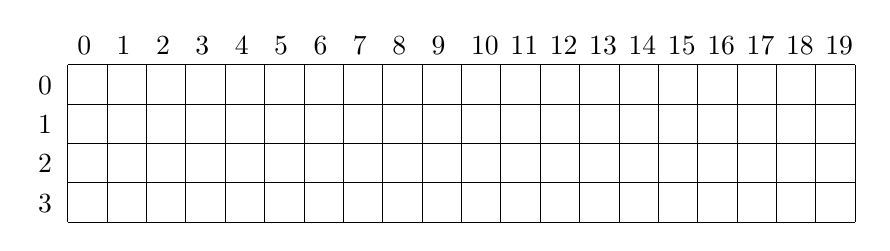
\begin{tikzpicture}
    \draw[step=0.5cm,black,very thin] (-5, -2) grid (5, 0);
    \foreach[count=\n from 0] \x in {-5, -4.5, ..., 4.5} {
      \draw (\x cm, 0) node[anchor=south west] {$\n$};
    }
    \foreach[count=\n from 0] \y in {-0.5, -1.0, ..., -2} {
      \draw (-5.5, \y) node[anchor=south west] {$\n$};
    }
  \end{tikzpicture}
  \caption{Схематическое изображение массива 4x20 (4 строки, 20 столбцов.)}
  \label{fig:2d-array-example}
\end{figure}

Можно также представить двумерный массив 4x20, как одномерный массив из 4-х
элементов, каждая ячейка которого содержит ссылку на ещё один одномерный массив
длиной 20 ячеек, как показано на
рис. \ref{fig:2d-array-example-with-references}.

\begin{figure}[ht]
  \centering
  \begin{tikzpicture}
    \draw[step=0.5cm,black,very thin] (-5, -2) grid (-4.5, 0);
    \draw[step=0.5cm,black,very thin] (-4, -2) grid (6, 0);
    \foreach[count=\n from 0] \x in {-4, -3.5, ..., 5.5} {
      \draw (\x cm, 0) node[anchor=south west] {$\n$};
    }
    \foreach[count=\n from 0] \y in {-0.5, -1.0, ..., -2} {
      \draw (-5.5, \y) node[anchor=south west] {$\n$};
    }
    \foreach[count=\n from 0] \y in {-0.25, -0.75, ..., -2} {
      \draw[{Circle}-{Stealth}]  (-4.8, \y) -- (-4, \y);
    }
  \end{tikzpicture}
  \caption{Схематическое представление массива 4x20 в виде одномерного массива
    из 4-х элементов со ссылками на одномерные массивы по 20 элементов.}
  \label{fig:2d-array-example-with-references}
\end{figure}

Для наших задач реализации игры нам потребуется задать массив, хранящий тип
данных \texttt{char}.  Размер нашего массива -- нашей игровой карты -- мы
зададим с помощью именованных констант, где-нибудь в глобальной области кода,
выше \texttt{setup}.

\begin{minted}{cpp}
  const int MAP_W = 20; // Ширина карты.
  const int MAP_H = 4;  // Высота карты.
\end{minted}

Далее создадим сам двумерный массив, который станет нашей игровой картой.

\begin{minted}{cpp}
  char game_map[MAP_H][MAP_W];
\end{minted}

Обратите внимание, что при объявлении массива используется две пары квадратных
скобок.  В первой паре скобок задаётся высота массива (количество строк), во
второй -- ширина массива (количество столбцов.)

Далее нам необходимо объявить функцию отображения карты на экране -- назовём её
\texttt{map\_show}.

\begin{minted}{cpp}
  void map_show() {
    for (int y = 0; y < MAP_H; y++) {
      for (int x = 0; x < MAP_W; x++) {
        lcd.setCursor(x, y);
        lcd.print( game_map[y][x] );
      }
    }
  }
\end{minted}

Как мы видим, тело функции состоит из двух вложенных друг в друга циклов
\texttt{for}.  Первый из циклов, идущий по \texttt{y}, перебирает строки
массива.  Второй цикл по \texttt{x} перебирает столбцы.  Поскольку цикл по
\texttt{x} вложен в цикл по \texttt{y}, то на каждое изменение \texttt{y}
происходит полный проход цикла по \texttt{x}.

Во вложенном цикле у дисплея вызывается функция \texttt{setCursor} для указания
позиции вывода символа на экран.  Далее символ печатается в указанную клетку
через \texttt{print}.

Поскольку массив \texttt{game\_map} имеет тип \texttt{char}, то символы,
хранящиеся в нём, автоматически выводятся на дисплей в правильном виде -- а
именно, как графические символы, а не их коды в таблице символов.

Функцию \texttt{map\_show} необходимо вызвать в \texttt{loop} для того, чтобы
карта отобразилась на экране.

\begin{minted}{cpp}
  void loop() {
    if (digitalRead(BUTTON_R) == LOW) {
      // ...
    }
    if (digitalRead(BUTTON_L) == LOW) {
      // ...
    }

    // Вызов функции отрисовки карты на экране дисплея.
    map_show();

    // Отрисовка игрока поверх карты.
    lcd.setCursor(player_x, player_y);
    lcd.print(PLAYER);

    // Задержка, чтобы избежать слишком быстрого считывания
    // нажатий на кнопки.
    delay(100);
  }
\end{minted}

Обратите внимание, что отрисовка карты выполняется перед отрисовкой игрока.
Если поменять этот порядок, то тогда игрок не будет виден на экране, ведь его
изображение будет перетёрто отрисовкой карты.

После загрузки и запуска данной программы вы можете обнаружить, что дисплей
наполнился случайными символами.  Это произошло потому, что мы не
инициализировали массив \texttt{game\_map} значениями, и там сейчас во всех
ячейках \emph{мусор} -- то есть, какие-то неожиданные значения.

Чтобы исправить эту ситуацию, нам необходимо создать функцию генерации карты,
которая будет заполнять карту чем-то вменяемым.  Для начала заполним карту
пробелами, которые будут у нас символизировать пустое место на карте.

В глобальной области перед \texttt{setup} зададим специальную константу для
обозначения пустого места.

\begin{minted}{cpp}
  const char SPACE = ' ';    // Пустое пространство.
\end{minted}

Теперь мы можем использовать константу \texttt{SPACE} для задания пустого места.

Перейдём к описанию функции генерации карты.

\begin{minted}{cpp}
  void map_generate() {
    for (int y = 0; y < MAP_H; y++) {
      for (int x = 0; x < MAP_W; x++) {
        game_map[y][x] = SPACE;
      }
    }
  }
\end{minted}

Как можно видеть, функция \texttt{map\_generate} не сильно отличается от функции
\texttt{map\_show}.

Функцию \texttt{map\_generate} необходимо вызвать один раз внутри функции
\texttt{setup}.

\begin{minted}{cpp}
  void setup() {
    lcd.init();
    lcd.backlight();

    // Настройка кнопок управления.
    pinMode(BUTTON_R, INPUT_PULLUP);

    // Вызов функции генерации карты.
    map_generate();
  }
\end{minted}

После загрузки новой прошивки в Arduino, мы должны увидеть экран, где
отображается только игрок, поскольку карта у нас ``пустая'' (заполнена
пробелами.)

Теперь мы получили возможность размещать на карте объекты.  Начнём с добавления
нового игрового объекта -- пусть это будет ``стена'', т.е. непроходимый участок
карты.  Зададим стену в виде символа ``\#''.

\begin{minted}{cpp}
  const char SPACE = ' ';    // Пустое пространство.
  const char WALL  = '#';    // Стена.
\end{minted}

После этого мы можем разместить этот объект на карте, модифицировав функцию
\texttt{map\_generate}.  Добавим несколько стен.

\begin{minted}{cpp}
  void map_generate() {
    for (int y = 0; y < MAP_H; y++) {
      for (int x = 0; x < MAP_W; x++) {
        game_map[y][x] = SPACE;
      }
    }

    // Добавляем вручную на карту объекты.
    game_map[0][10] = WALL;
    game_map[1][10] = WALL;
    game_map[2][10] = WALL;
  }
\end{minted}

\end{document}
